%保存为UTF-8编码格式
%用xelatex编译
 
\documentclass[UTF8,a4paper,12pt]{ctexart}
\usepackage[left=2.50cm, right=2.50cm, top=2.50cm, bottom=2.50cm]{geometry} %页边距
\CTEXsetup[format={\Large\bfseries}]{section} %设置章标题字号为Large,居左
\CTEXsetup[format={\Large\bfseries}]{subsection} %设置章标题字号为Large,居左
\CTEXsetup[format={\Large\bfseries}]{subsubsection} %设置章标题字号为Large,居左
%\CTEXsetup[number={\chinese{section}}]{section}
%\CTEXsetup[name={(,)}]{subsection}
%\CTEXsetup[number={\chinese{subsection}}]{subsection}
%\CTEXsetup[name={(,)}]{subsubsection}
%\CTEXsetup[number=\arabic{subsubsection}]{subsubsection}  %以上四行为各级标题样式设置,可根据需要做修改

%\linespread{1.5} %设置全文行间距
 
 
%\usepackage[english]{babel}
%\usepackage{float}     %放弃美学排版图表
\usepackage{fontspec}   %修改字体
\usepackage{amsmath, amsfonts, amssymb} % 数学公式相关宏包
\usepackage{color}      % color content
\usepackage{graphicx}   % 导入图片
\usepackage{subfigure}  % 并排子图
\usepackage{url}        % 超链接
\usepackage{bm}         % 加粗部分公式,比如\bm{aaa}aaa
\usepackage{multirow}
\usepackage{booktabs}
\usepackage{epstopdf}
\usepackage{epsfig}
\usepackage{longtable}  %长表格
\usepackage{supertabular}%跨页表格
\usepackage{algorithm}
\usepackage{algorithmic}
\usepackage{changepage}
\usepackage{hyperref}
\usepackage[square, comma, sort&compress, numbers]{natbib}
\usepackage{appendix}
\usepackage[final]{pdfpages}% 插入pdf封面。
%%%%%%%%%%%%%%%%%%%%%%%
% -- text font --
% compile using Xelatex
%%%%%%%%%%%%%%%%%%%%%%%
% -- 中文字体 --
%\setCJKmainfont{Microsoft YaHei}  % 微软雅黑
%\setCJKmainfont{YouYuan}  % 幼圆
%\setCJKmainfont{NSimSun}  % 新宋体
%\setCJKmainfont{KaiTi}    % 楷体
\setCJKmainfont{SimSun}   % 宋体
%\setCJKmainfont{SimHei}   % 黑体
 
% -- 英文字体 --
\setmainfont{Times New Roman}
%\setmainfont{DejaVu Sans}
%\setmainfont{Latin Modern Mono}
%\setmainfont{Consolas}
%
%
\renewcommand{\algorithmicrequire}{ \textbf{Input:}}     % use Input in the format of Algorithm
\renewcommand{\algorithmicensure}{ \textbf{Initialize:}} % use Initialize in the format of Algorithm
\renewcommand{\algorithmicreturn}{ \textbf{Output:}}     % use Output in the format of Algorithm
\renewcommand{\abstractname}{\textbf{\large {摘\quad 要}}} %更改摘要二字的样式
\newcommand{\xiaosi}{\fontsize{12pt}{\baselineskip}}     %\xiaosi代替设置12pt字号命令,不加\selectfont,行间距设置无效
\newcommand{\wuhao}{\fontsize{10.5pt}{10.5pt}\selectfont}
 
\usepackage{fancyhdr} %设置全文页眉、页脚的格式
\pagestyle{fancy}
\lhead{}           %页眉左边设为空
\chead{}           %页眉中间
\rhead{}           %页眉右边
%\rhead{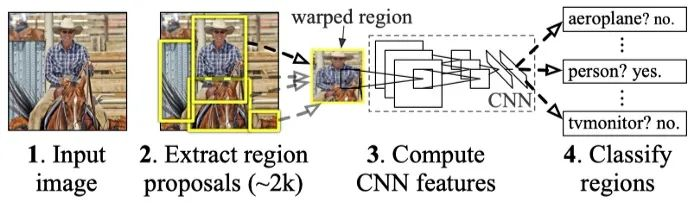
\includegraphics[width=1.2cm]{1.eps}}  %页眉右侧放置logo
\lfoot{}          %页脚左边
\cfoot{\thepage}  %页脚中间
\rfoot{}          %页脚右边
 
 
%%%%%%%%%%%%%%%%%%%%%%%
%  设置水印
%%%%%%%%%%%%%%%%%%%%%%%
%\usepackage{draftwatermark}         % 所有页加水印
%\usepackage[firstpage]{draftwatermark} % 只有第一页加水印
% \SetWatermarkText{Water-Mark}           % 设置水印内容
% \SetWatermarkText{\includegraphics{fig/ZJDX-WaterMark.eps}}         % 设置水印logo
% \SetWatermarkLightness{0.9}             % 设置水印透明度 0-1
% \SetWatermarkScale{1}                   % 设置水印大小 0-1
 
\usepackage{hyperref} %bookmarks
\hypersetup{colorlinks, bookmarks, unicode} %unicode
 
 
 
\title{\textbf{\Large{MobileNet系列论文阅读分析}}}
\author{ 崔虎\thanks{贵州大学,计算机科学与技术学院,软件工程2019021932} }
\date{2020年9月12}
 
 
 
\begin{document}
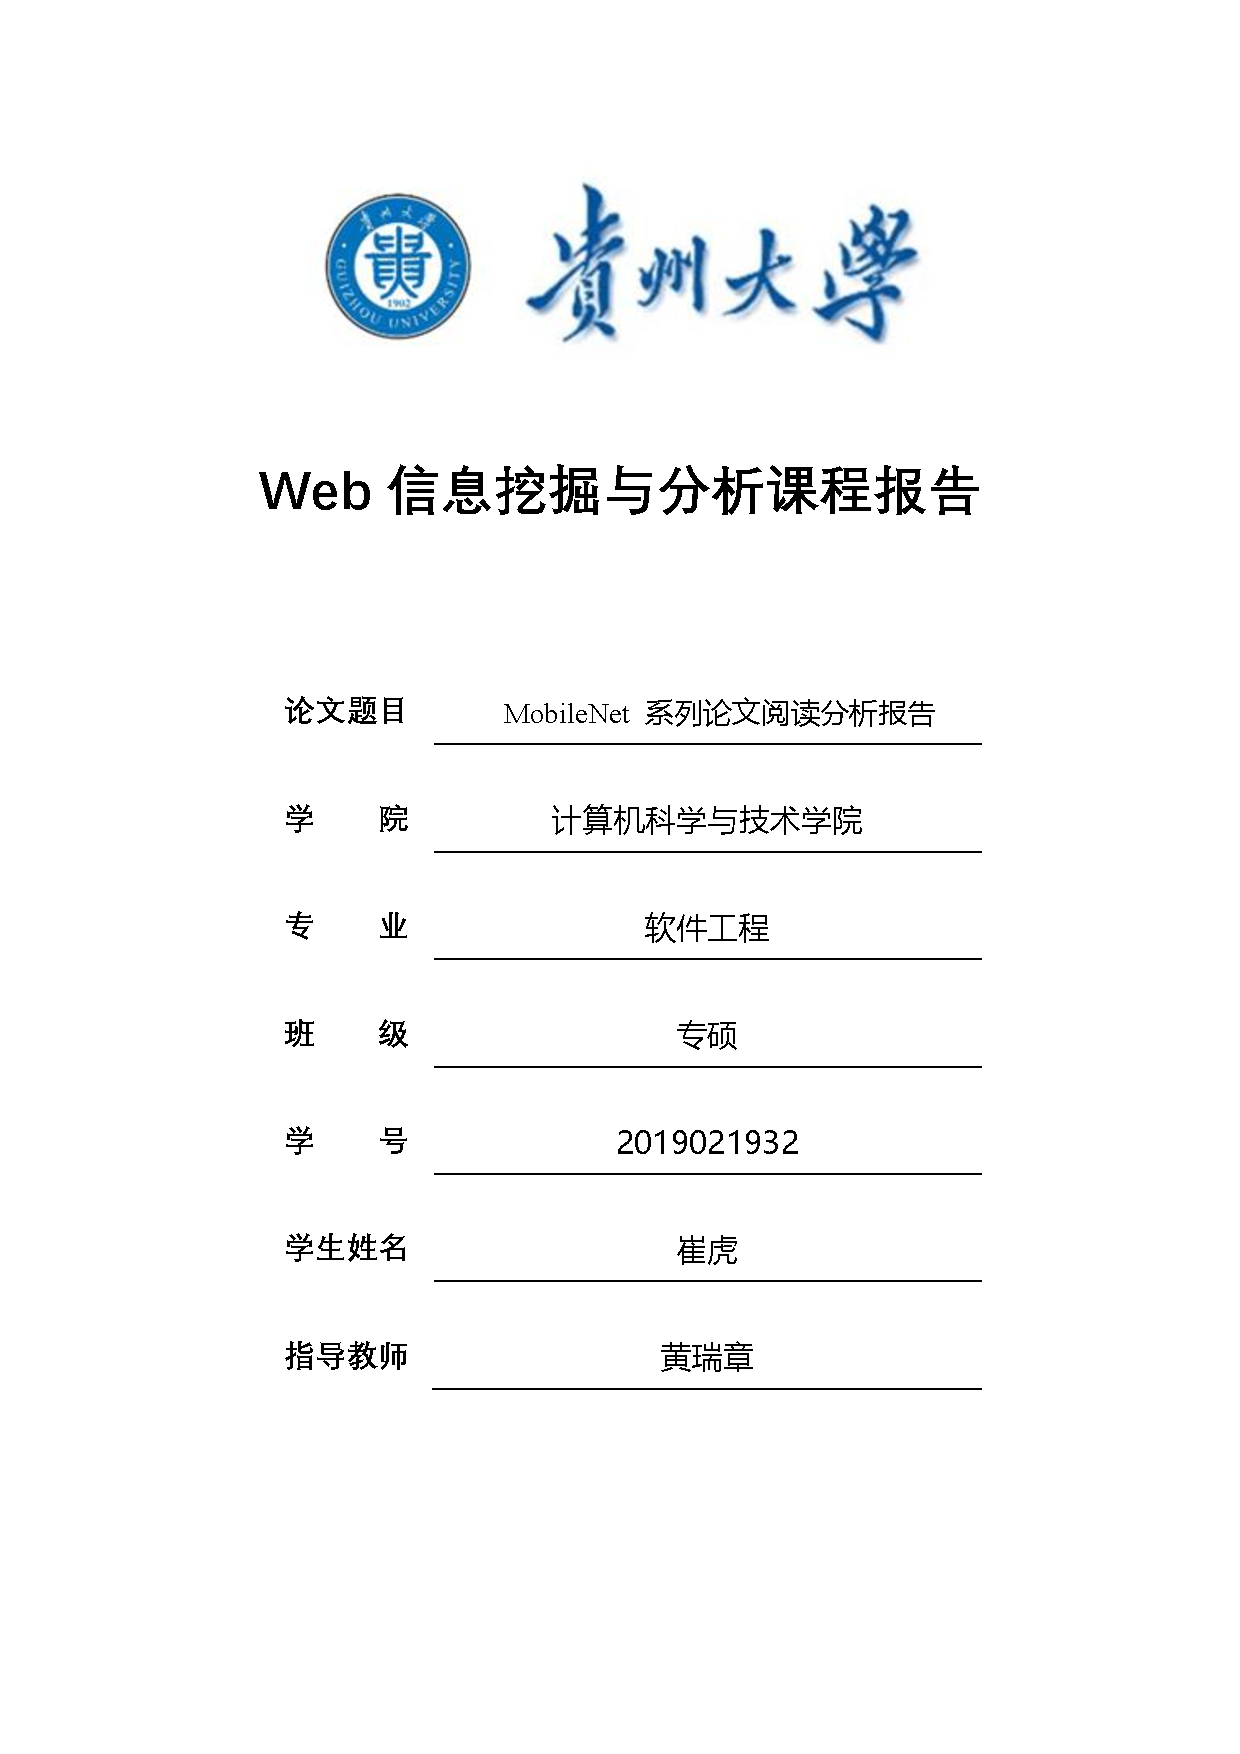
\includepdf{课程报告封面建议模板.pdf} 
\newpage


\tableofcontents
\maketitle
%\tableofcontents
 
\begin{abstract}
{\kaishu 神经网络的快速发展使得人工智能领域产生了革命性的变化,比如图像分类和识别的精度已经超越了人类本身的识别精度,语义分隔,物体检测,图像生成等等有意思而又有意义的工作都会在每年的计算机顶级会议中出现,而这一切的基础都是因为我们计算机的计算能力在近些年有了极大的提高,然而,我们也经常发现,很多计算模型虽然很有意思,却过分依赖于硬件基础。而本文所分析的三篇MobileNet系列论文,就是针对如何使得原本重量型的模型应用于移动和嵌入端的问题,来展开讨论和分析。}
\end{abstract}
 
\begin{center}
\large{\textbf{Abstract}}
\end{center}
 
\begin{adjustwidth}{1cm}{1cm}
\hspace{1.5em}The rapid development of neural network makes a revolutionary change in the field of artificial intelligence. For example, the accuracy of image classification and recognition has exceeded the recognition accuracy of human beings. Interesting and meaningful work will appear in the top computer conference every year, and the foundation of all these is because of our computer Computing power has been greatly improved in recent years. However, we often find that many computing models, although interesting, rely too much on hardware. The three papers in this paper are about how to apply the original weight model to the mobile and embedded end.
\end{adjustwidth}
 
\thispagestyle{empty}       %本页不显示页码
\newpage                    %分页
%\tableofcontents\thispagestyle{empty}
\newpage
\setcounter{page}{1}        %从下面开始编页,页脚格式为导言部分设置的格式
 
 
\section{MobileNetV1}
\bibliographystyle{plain}
	该论文是2017年由谷歌团队发表\cite{2017MobileNets}, 提出了一类高效的移动和嵌入式视觉应用模型MobileNets。MobileNets基于一种流线型结构,它使用深度可分离卷积来构建轻量化的深度神经网络。引入了两个简单的全局超参数,它们可以有效地在延迟和准确性之间进行权衡。这些超参数允许模型生成器根据问题的约束为其应用程序选择适当大小的模型。
	
	我们以下就论文中的两个重点进行分析:{\heiti 流线型结构(深度分离卷积)与全局超参数}。
\subsection{工作基础}
		mobilenet主要由深度可分离卷积构建,最初在\cite{2014Rigid}中引入,随后在初始模型\cite{2015Batch}中使用,以减少前几层的计算量。Flattened networks\cite{2014Flattened}利用全因子卷积构建网络,并展示了极大因子分解网络的潜力。随后,Exception network\cite{2016Xception}演示了如何扩展深度可分离滤波器,以超越初始V3网络。另一个小型网络是Squeezenet\cite{DBLP:journals/corr/IandolaMAHDK16},它使用bottleneck方法来设计一个非常小的网络。其他减少计算量的网络包括 structured transform network\cite{2015Structured}和deep fried convnets\cite{2015Deep}。
		
 另一种获得小网络的方法是收缩、分解或压缩预训练网络。基于乘积量化的压缩\cite{36},基于哈希\cite{2},霍夫曼编码\cite{5};此外,此外,还有各种因子分解来加速预训练网络\cite{14,20}。另一种训练小网络的方法是蒸馏\cite{9},用较大的网络来teach小网络。还有一种方法比较新兴,称为low bit networks\cite{4,22,11}。
 
 
 \subsection{深度可分离卷积}
 
 深度可分离卷积是MobileNet的基础,它与普通卷积的区别主要在于结构,而正式这种结构,导致了网络参数的大幅度下降与模型推理速度的大幅度提高,
 
 \begin{figure}[htpb]
 	\subfigure[传统卷积]{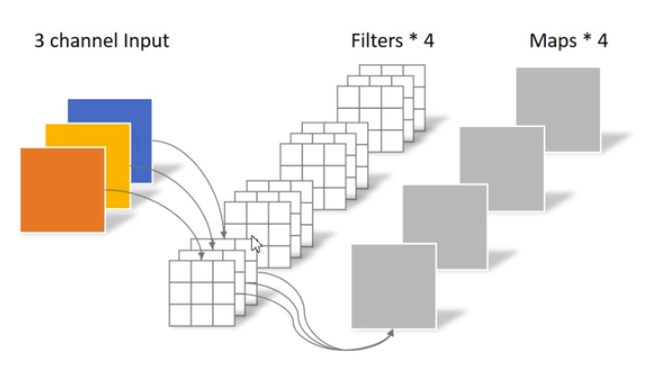
\includegraphics[width=0.4\linewidth]{webmin/ctjj.png}\label{fig-chuangtongjuanji}}
%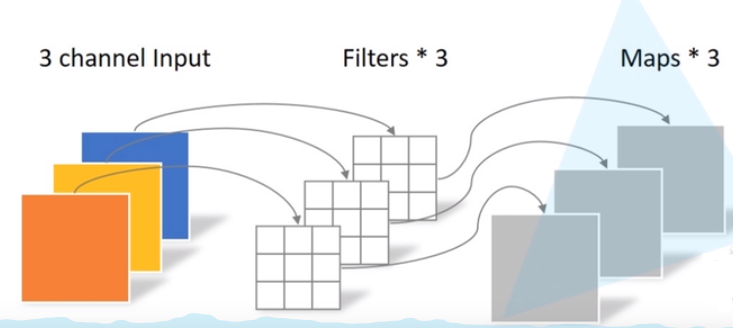
\includegraphics[width=\linewidth]{imagefile
\hskip2em
\subfigure[DP卷积]{\includegraphics[width=0.4\linewidth]{webmin/dpwd.png}\label{fig-detpwise}\label{fig-dpjuanji}}

\caption{传统卷积与depthwise卷积对比}

\label{fig-juanjiduibi}
 \end{figure}

从图上我们可以看出传统卷积与深度可分离卷积(Depthwise Separable Convolution)的不同。假设我们的输入图像为3通道,尺寸是假设为$D \times D$经过stride=1卷积后,假设卷积核为$K \times K $要产生n通道卷积,那么我们传统卷积计算量是:
\begin{equation}
	C1 = 3 \times D \times D \times K \times K \times n
	\label{eq-chuantongjisuanliang}
\end{equation}
 
那么以相同的尺度,要输出相同的通道和尺寸的特征图,Depthwise Separable Convolution 的计算量又是多少呢?

从图\autoref{fig-dpjuanji} 可以看出,dp卷积相对于传统卷积,是分两步走的,按原论文中的意思是,第一进行图像滤波,第二部进行特征生成,第一步先对原来三通道图像的三个通道\emph{分别进行卷积},生成的中间结果我们可以看出依然是三通道的。
第二部对生成的三通道的中间结果进行$1 \times 1$ 卷积核,n——outchannel,生成输出特征图。

第一步的计算量:
\begin{equation}
D \times D \times K \times 	K \times 3 
\label{eq-diyibu}
\end{equation}
第二部计算量:
\begin{equation}
	D \times D \times 1 \times 1 \times n
	\label{eq-dierbu}
\end{equation}

我们将式\ref{eq-diyibu}和式\ref{eq-dierbu}相加,得到:
\begin{equation}
	C2 = D \times D \times K \times 	K \times 3 + D \times D \times 1 \times 1 \times n
	\label{eq-zongjisuanliang}
\end{equation}

然后我们对比以下dp卷积和传统卷积的计算量:
\begin{equation}
	d = \frac{3 \times D \times D \times K \times K \times n}{D \times D \times K \times 	K \times 3 + D \times D \times 1 \times 1 \times n}
	\label{eq-bili}
	\end{equation}
从式\ref{eq-bili} 可以看出,当我们假设卷积核等于3的时候,这个比值十分等于$\frac{1}{n} + \frac{1}{27}$ 的倒数,可以看到,这个计算量和参数量的区别是十分巨大的,而得到的却都是同样通道的特征图。

\subsection{网络结构}
我们现在来具体看看实际的Mobilnet的网络结构:
\begin{figure}[htbp]
	\centering
	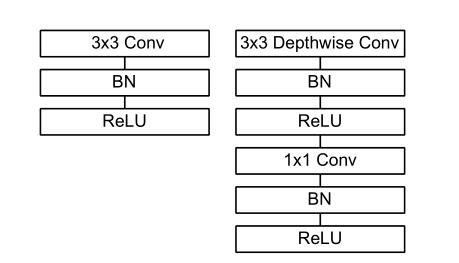
\includegraphics[width=0.5\linewidth]{webmin/juanjistr.jpg}
	\caption{左:batchnorm和标准卷积层
		线性整流函数(Rectified Linear Unit)右:深度可分离的卷积,深度和点态层,然后是批范数和ReLU。}
	\label{fig-duibi}
\end{figure}
如图\ref{fig-duibi}所示,右图即为即为深度可分离卷积的模块,我们称其为 {\heiti Conv dw} 卷积。

我们再来看看在Conv dw 基础上实现实现的整个Mobilenet Net 结构:
\begin{figure}[htpb]
	\centering
	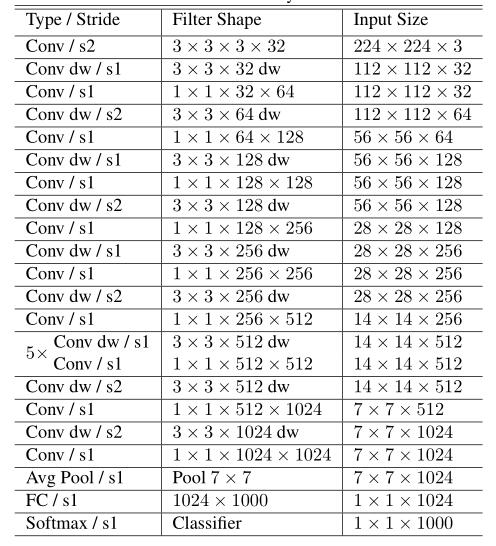
\includegraphics[width=0.5\linewidth]{webmin/netstr.jpg}
	\caption{MobileNet 主体架构}
	\label{fig-wangluojiegou}
\end{figure}
我们可以从\ref{fig-wangluojiegou}看到网络主要有四种结构,Conv1-1,Conv dw 3-3,Conv 3-3, Full Connected。\\
论文中分析了网络中这四种结构的参数和计算量对比:
\begin{figure}[htpb]
	\centering
	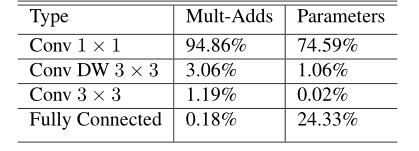
\includegraphics[width=0.5\linewidth]{webmin/计算量对比.jpg}
	\caption{每层网络资源情况}
	\label{fig-ziyuan}
\end{figure}

从图\ref{fig-ziyuan}可以看出计算资源和参数大都几种到了conv1-1和全连接层了。

\subsection{超参$\aleph$和$\rho$}\label{sec-chaocan}

\subsubsection{窄网络}
该论文的另一个亮点,则是提出两个超参数$\alpha$和$\rho$,我们不禁要问这两个参数是做什么的呢?论文中给出的解释是Tinner MOdell和Reduced Representation,大致意思就是为了更‘瘦’的模型,和‘多分辨率’效果。\\
我们从图\ref{fig-canshuhexiaoguoduibi}可以看出,在conv MobileNet和 conv dw Mobilenet 的对比中,采用了conv dw 卷积的网络的参数和计算量(Mult-adds) 下降了接近八倍之多。
\begin{figure}[tbph]
	\centering
	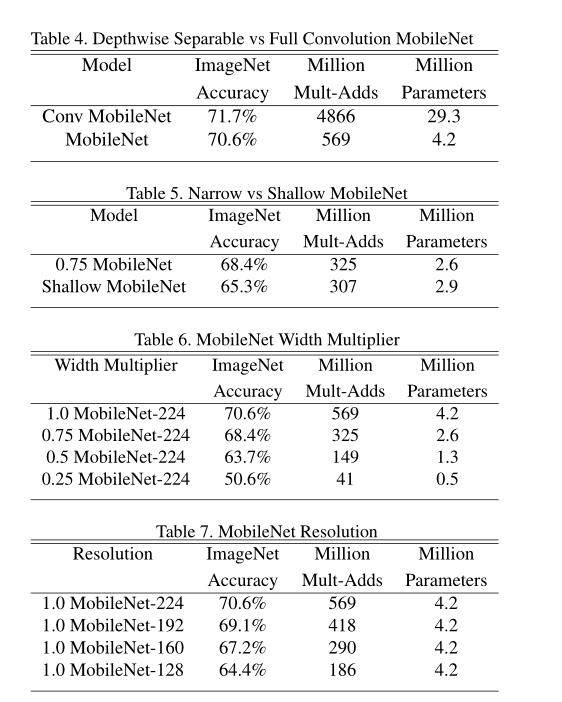
\includegraphics[width=0.5\linewidth]{webmin/参数对比图.jpg}
	\caption{参数和效果对比图}
	\label{fig-canshuhexiaoguoduibi}
\end{figure}

那么如果如果遇到一种情况,也就是将即便参数下降了这么多,还是显得太大,还是无法适应我们的目标平台,怎么?这也就两个超参数$\alpha$ 和 $\rho$ 的作用了。

\begin{equation}
	D_{K} \cdot D_{K} \cdot \alpha M \cdot D_{F} \cdot D_{F}+\alpha M \cdot \alpha N \cdot D_{F} \cdot D_{F}
\label{eq-alba}
\end{equation}

式\ref{eq-alba}中,$\alpha \in(0,1]$ , 一般设为1,0.75,0.5,0.25,它是用来空值通道数M,N的,M为输入通道,N为输出通道,我们从图\ref{fig-canshuhexiaoguoduibi}可以看出,$\alpha=0.75$和$\alpha=1.0$的时候,精度从70.6\%降低到了68.4\%,而参数和计算量降低了近乎一半。论文中将这种降低通道的数的方法成为{\heiti 窄网络}。而将减少网络深度的网络成为{\heiti 浅网络}。

同样我们可以从图\ref{fig-canshuhexiaoguoduibi}中可以看出,0.75的窄网络和浅网络的对比,在参数和计算量相当的情况下,宅网络要比浅网络准确度表现更好。


\subsubsection{多分辨率效果}
$\alpha$用控制卷积通道数的方法来控制参数,使得在准确度下降不高的情况下,进一步降低网络的计算量和参数量,而$\rho$则是用来控制图像输入尺度的。

\begin{equation}
	D_{K} \cdot D_{K} \cdot \alpha M \cdot \rho D_{F} \cdot \rho D_{F}+\alpha M \cdot \alpha N \cdot \rho D_{F} \cdot \rho D_{F}
	\label{eq-ro}
\end{equation}
式\ref{eq-ro}就是完整的超参控制公式。当然超参数$\rho$ 一般是直接手动的来进行控制输入图像的大小尺度即可,从图\ref{fig-canshuhexiaoguoduibi}最后一表可以看出,不同尺度的准确率和相应的参数和计算量情况。 

\subsection{与其他卷积网络框架对比}


 
论文中,将MobileNet作为bacbone骨干网络部署到目标检测框架中,并且根据当年COCO挑战赛的报告数据进行了对比,MobileNet在faster-RCNN\cite{23}和SSD\cite{21}框架下与VGG和Inception V2\cite{13}进行了比较。,SSD被评估为300输入分辨率(ssd300),faster-RCNN与300和600输入分辨率(FasterRCNN 300,FasterRCNN 600)进行了比较。更快的RCNN模型评估每个图像300个RPN建议框。

对于这两种框架,MobileNet在计算复杂度和模型大小上与其他网络相比具有可比性。
 
\begin{figure}[htbp]
	\centering
	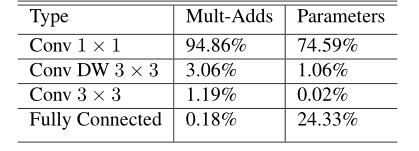
\includegraphics[width=0.5\linewidth]{webmin/计算量对比.jpg}
	\caption{使用不同框架和网络架构的COCO对象检测结果比较}
	\label{fig-mubiaokuangjiaduibi}
\end{figure}

\begin{figure}[htbp]
	\centering
	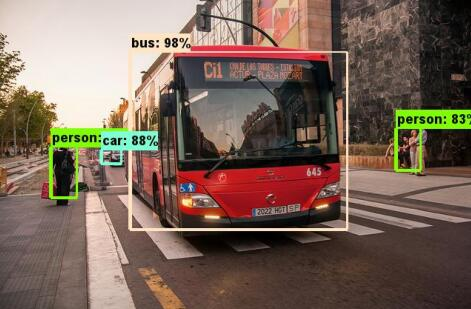
\includegraphics[width=0.5\linewidth]{webmin/ssd示例.jpg}
	\caption{以MobileNet为骨干网络的SSD示例}
	\label{fig-ssd}
\end{figure}
我们从图\ref{fig-mubiaokuangjiaduibi}可以看出,MAP指标(AP at IoU=0.50:0.05:0.95) 相比其他骨干网络的目标检测框下降了一到三个百分点,但是计算量和参数量大小却比他们少5-10倍,这显然是值得的。
 
 
 
\subsection{小结}
经过我们仔细的阅读这篇论文,我们得知了作者是如何通过引入新的卷积DW卷积来代替传统卷积,同时引入两个超参数来对模型的参数和计算量进行控制,在将计算量和参数量与准确度之间进行权衡,以达到可以将模型运用于嵌入式或者移动平台。

然而,方法虽然有效,但是经过测试,有人发现dw网络中的图\ref{fig-duibi}conv1$\times$1卷积的梯度很容易便程0,导致损失损失很多信息。
 
 
 
 
 
 
 
 
\section{MobileNetV2}\label{sec-v2}
MobileNetv2网络模型是2018年谷歌团队在v1基础上提出的\cite{MOBV2},主要引入了两个改动,Linear Bottleneck 和 Inverted Residual Blocks.也就是线性Bottleneck和反残差网络。所以,我们分析的重点也就几种在这两个部分。


\subsection{Linear BottelNeck的提出}

在分析LinearBottelNeck的时候,我们需要先分析以下Relu激活函数\ref{fig-relu}的作用,一般用它来代替sigmod函数,因为sigmod激活函数很容易引起梯度消失或者梯度爆炸。然而Relu的激活张量如果应用于低纬度可能会使得原本的输入信息出现丢失。
\begin{figure}[htbp]
	\centering
	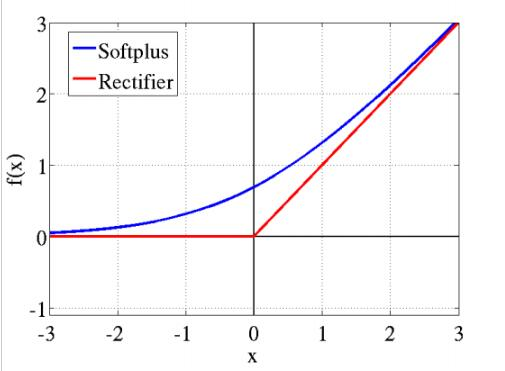
\includegraphics[width=0.5\linewidth]{webmin/relu.jpg}
	\caption{Relu函数}
	\label{fig-relu}
\end{figure}


\begin{figure}[htbp]
	\centering
	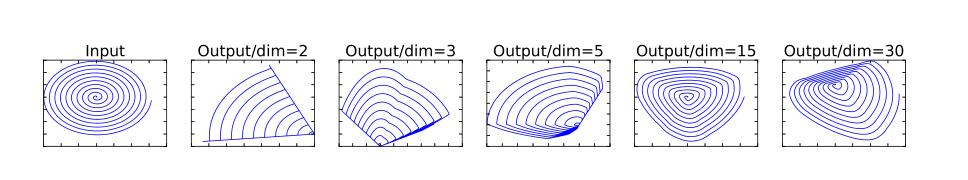
\includegraphics[width=\linewidth]{webmin/relu维度信息.jpg}
	\caption{Relu不同维度应用后还原后得到的信息量对比}
	\label{fig-reluxinxi}
\end{figure}


从图\ref{fig-reluxinxi}可以看出,当relu函数应用于低纬度特征下后,经过信息还原,信息丢失了很多,而当特征维度越来越高,应用relu激活张量后,还原后,保留的信息就越多,论文中称这种高纬度的relu激活近似为线性,因为信息没有或者丢失的很少。说的直白点,就是通道数数越多,经过relu后,在一个通道上丢失的信息可能在别的通道上保留着,这样将最后的结果进行叠加,那么丢的信息也就微乎其微了。


而瓶颈层又于rule激活张量的这些特性有什么关系呢?我们从上边的分析得出,越是高维,利用rule激活保留的信息越接近于线性,那么我们如果遇到这种情况:输入的感兴趣的信息是低维的,该怎么办?不能用relu激活张量了嘛?很简单,将输入信息提升到高维,然后使用relu,之后再进行降维到我们的目标维度即可。论文中将这种方法成为BottleNeck。这相对于mobilenetv1来说是一个很明显的提升。

\subsection{反残差 Inverted residuals}


 \begin{figure}[htbp]
 	\centering
 	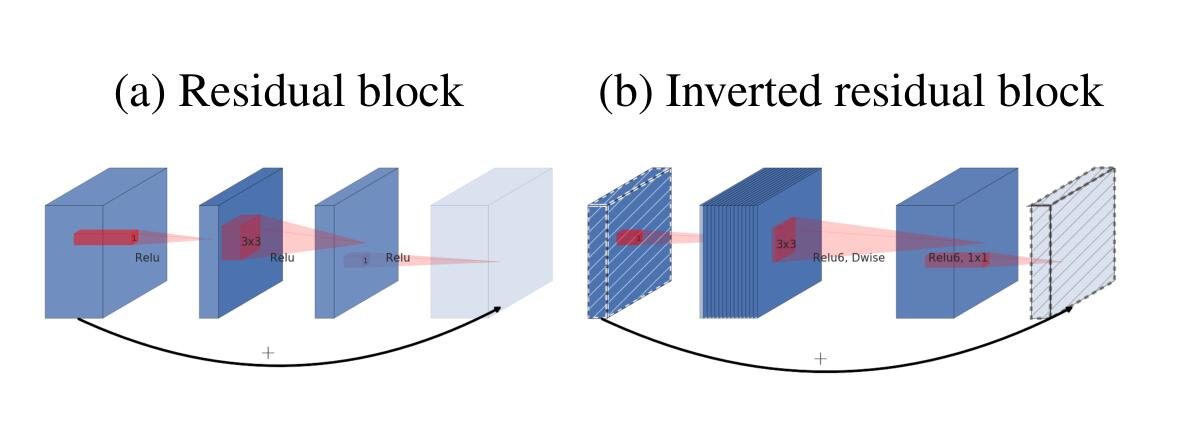
\includegraphics[width=\linewidth]{webmin/残差于反残差.jpg}
 	\caption{残差于反残差对比}
 	\label{fig-canchaduibi}
 \end{figure}
 
 从图\ref{fig-canchaduibi}可以看出,残差\cite{resnet,renet2}于反残差结构的对比,残差块是在多通道上进行叠加,反残差正好相反,是在低通道上进行叠加,通过残差链接,特征图可以总和不同尺度的特征,那么反残差块呢?通道数降低了是否也能达到综合不同尺度特征的效果呢?这就要结合我们之前所说的BottleNeck,bottleneck的结构正好就是中间维度高,两端维度低,并且可以线性的保留信息。正好于反残差完美结合。
 
 \begin{figure}[htbp]
	\centering
	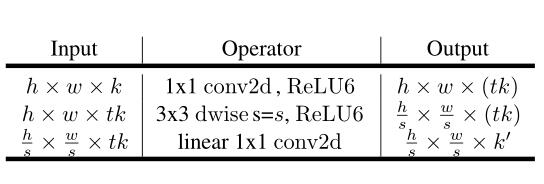
\includegraphics[width=\linewidth]{webmin/反残差瓶颈块.jpg}
	\caption{反残差瓶颈块}
	\label{fig-fancanchapingjing}
\end{figure}
 
 将relu的高纬特性,和反残差结构组合起来,就得到了Bottleneck residual block ,结构网络结构如图\ref{fig-fancanchapingjing}所示,与MobileNetV1中的dp卷积块不同,这里先使用$1\times1 $的卷积对输入图像尺度为 $ h \times w \times k$的张量进行维度的提升,以方便relu激活张量可以保持线性而不丢失信息,其中的 t 是维度扩展因子,然后第二步使用$3 \times 3$dw 卷积,对 $tk$个通道分别使用$k=3 \times 3, stride=s $的卷积,对张量进行滤波处理,然后使用$1 \times 1$ 的卷进行降维度处理。
 
我们还注意到,前两部卷积后使用的都是Relu6 激活函数,relu6与relu激活函数的不同在于后者的范围是$ 0 \to \infty$,而前者的激活范围是$0 \to 6$,在移动端或者嵌入式端,float16下,可以精确描述数据精度,否则范围太大,无法描述大范围的数值,效果反倒不好。

对于扩展因子 $t$,论文中描述,一般取值在$5 \to 10$即可。

  \begin{figure}[htbp]
 	\centering
 	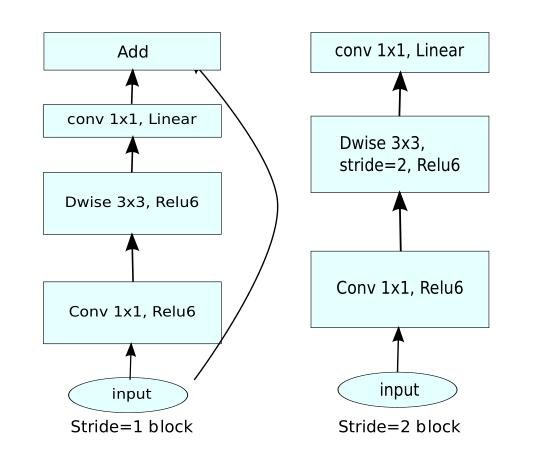
\includegraphics[width=0.5\linewidth]{webmin/mobnet.jpg}
 	\caption{MobilenetV2}
 	\label{fig-mobnet}
 \end{figure}
 
 最后的BottleNeck卷积块,如图\ref{fig-mobnet}所示,左边为有残差链接的块,右边为无残差链接的块,结合图\ref{fig-mobnetjiegou}可以看出,只有在每个上层卷积组的时候,stride=2,每个卷积块层的内部图像的尺度是不变的,stride=1,也就是图\ref{fig-mobnet}中的右图是为了缩放张量尺度,而残差层都是在每个卷积块的内部的。
 

 
  \begin{figure}[htbp]
 	\centering
 	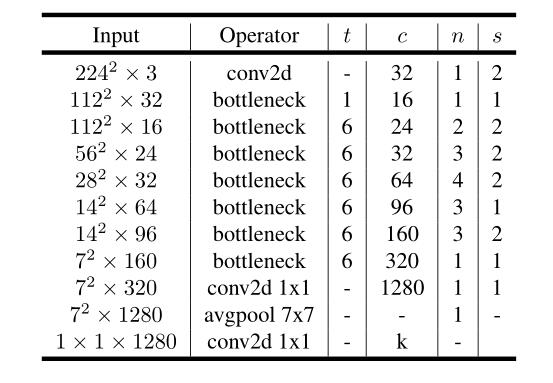
\includegraphics[width=0.5\linewidth]{webmin/v2架构图.jpg}
 	\caption{MobilenetV2整体网络结构}
 	\label{fig-mobnetjiegou}
 \end{figure}
 
从图\ref{fig-mobnetjiegou}可以看出,标准输入是224,通道数为3的图像,其中t表示膨胀系数,c表示卷积输出通道,n表示每个卷积层内部的bottleneck块重复次数,s表示每个卷积层第一个bottleneck块的卷积stride大小。
 
 
 \subsection{效果比较}
 
 
  \begin{figure}[htbp]
 	\centering
 	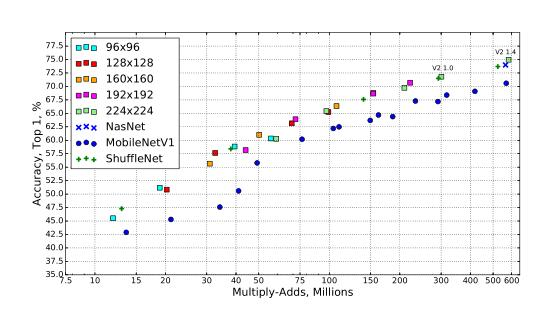
\includegraphics[width=0.5\linewidth]{webmin/不同分辨率.jpg}
 	\caption{不同网络在图像分类方面的比较}
 	\label{fig-tuxiangfenlei}
 \end{figure}
 
 
   \begin{figure}[htbp]
 	\centering
 	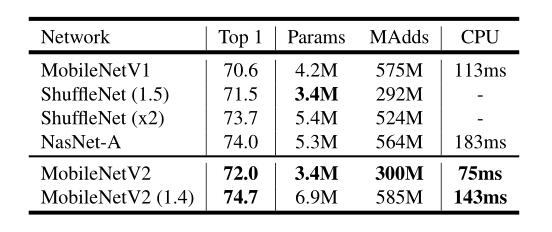
\includegraphics[width=0.5\linewidth]{webmin/不同分辨率2.jpg}
 	\caption{不同网络在图像分类方面的比较}
 	\label{fig-tuxiangfenlei2}
 \end{figure}
 
 图\ref{fig-tuxiangfenlei}对不同设置不同的超参数\ref{sec-chaocan}的mobileNetv2网络与NasNet\cite{NasNet},ShuffleNet\cite{ShuffleNet},\\MobileNetV1\cite{2017MobileNets}在图像分类效果上的比较。横轴表示计算量,纵轴表示准确率,可以看出计算量相当情况下MobileNetV1的效果已经有所落后了,但是我们可以看出,MobileNetV2的设置不同超参$\aleph$和$\rho$的情况下,效果均好于其他网络。从图\ref{fig-tuxiangfenlei2}也可以看出,相比于其他移动网络,MobileNetV2的推理速度更块。
 
 该论文实验部分另一个亮点,个人认为是将SSD\cite{21}网络进行修改部分,不仅是用MobileNetV2来替换其骨干网络,而且将其预测部分的卷积网络替换为BottleNet卷积,使得模型更加轻量化,论文中称该版本为SSDLite。
 
 
 \begin{figure}[htbp]
 	\centering
	 	\subfigure[]{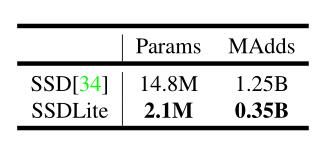
\includegraphics[width=0.4\linewidth]{webmin/ssdlite1.jpg}\label{fig-ssd1}}
 	\quad
 	\subfigure[]{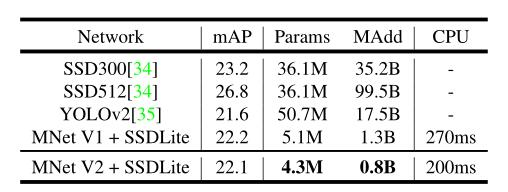
\includegraphics[width=0.4\linewidth]{webmin/ssdlite2.jpg}\label{fig-ssd2}}
 	\caption{SSDlite效果比较}
 	\label{fig-ssdlite}
 \end{figure}
 
 从图\ref{fig-ssd1}中,我们可以看出,SSDlite相比于SSD\cite{21},参数量下降了近七倍,计算量下降了近四倍。
 从图\ref{fig-ssd2}中,看出,无论是参数量还是计算量或者推理速度,效果也比YOLOV2\cite{YOLO9000}好。
 
 \subsection{小结}
 MobileNetV2最难理解的其实是 Linear Bottlenecks,论文中用很多公式表达这个思想,但是实现上非常简单,就是在 MobileNetV2 微结构中第二个 PW 后无 ReLU6。对于低维空间而言,进行线性映射会保存特征,而非线性映射会破坏特征,而Bottelnecks就是用维度提升然后relu,然后降维的方法实现本来是低纬度的relu线性转换。
 
 
 
 
 
\section{MobileNetV3}
最后一篇论文同样是谷歌团队19年发表的题名为《Searching for MobileNetV3》\cite{MobV3}的论文,顾名思义,V3 网络是利用搜索技术来得到模型。该论文的两大创新点:
\begin{enumerate}
	\item 互补搜索技术组合:由资源受限的NAS\cite{NasNet}执行模块级搜索,NetAdapt\cite{NetAdapt}执行局部搜索。
	\item  网络结构改进:将最后一步的平均池化层前移并移除最后一个卷积层,引入h-swish激活函数。
\end{enumerate}

\subsection{结构特点}

 \begin{figure}[htbp]
	\centering
	\subfigure[]{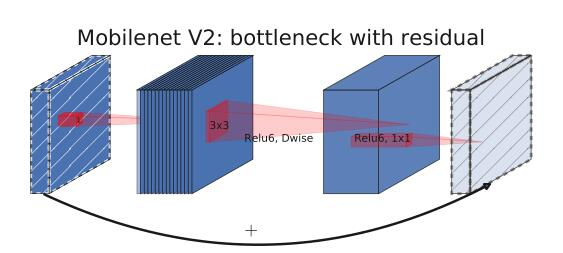
\includegraphics[width=0.4\linewidth]{webmin/v2.jpg}\label{fig-v2}}
	\quad
	\subfigure[]{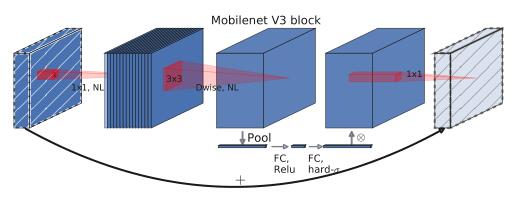
\includegraphics[width=0.4\linewidth]{webmin/v3.jpg}\label{fig-v3}}
	\caption{MobileNetV3 block}
	\label{fig-MobileNetV3 block}
\end{figure}

从图\ref{fig-MobileNetV3 block}可以看出MobileNetV3 block相对MobileNetV2 block的变化,它用了MobileNetV1\cite{2017MobileNets}的深度可分离卷积(depthwise separable convolutions)、MobileNetV2\cite{MOBV2}的具有线性瓶颈的逆残差结构(the inverted residual with linear bottleneck)和MnasNet\cite{MnasNet}的基于squeeze and excitation结构的轻量级注意力模型。MobileNetV3正式综合以上三种网络设计结构而完成的。

\subsection{互补网络搜索}
个人认为网络搜索是本论文的基础,因为从论文中我们得知,网络的各个模块都是应用NAS\cite{MnasNet}搜索得到的,那么网络搜索究竟是什么东西呢?之前有甚多新颖的网络,比如ResNet\cite{resnet,renet2},ShuffleNet\cite{ShuffleNet,ShuffleNet2}等,都是通过研究人员手工设计出来的,但是随着神经网络越来越复杂,设计网络的时间成本和试错成本越来越难以让人接受,而网络搜索就是解决这个难题的,简单来说就是应用类似强化学习的方法,在给定的搜索空间中,依照某种搜索策略进行网络的部件搜索,产生一个网络,然后对这个网络进行评估,循环不断的进行,直到生成最优的网络。

 \begin{figure}[htbp]
	\centering
	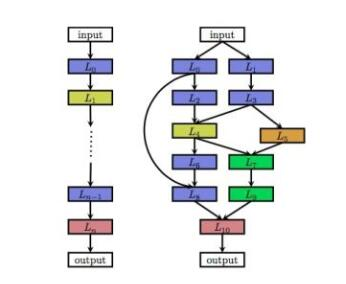
\includegraphics[width=0.5\linewidth]{webmin/网路搜索.jpg}
	\caption{网络搜索示例}
	\label{fig-wangluosousuo}
\end{figure}
从\ref{fig-wangluosousuo}可以看出,网络搜索的简单例子,可以将搜索空间设定为组成网络的各种基本层,也可以设定称基本块,甚至还允许网络进行分割和残差链接。

而在改论文中,用的就是一种互补网络搜索的方法,作者结合了两种策略,资源受限的NAS(platform-aware NAS)\cite{MnasNet},NetAdapt\cite{NetAdapt},前者用于计算和参数量受到限制的前提下搜索网络的各个模块,所以称之为模块级搜索,后者用于对各个模块确定之后的网络,进行微调,也就是参数和层级级别搜索。从而达成互补性搜索。


\subsection{网络的改进于h-swish}

\begin{figure}[htbp]
	\centering
	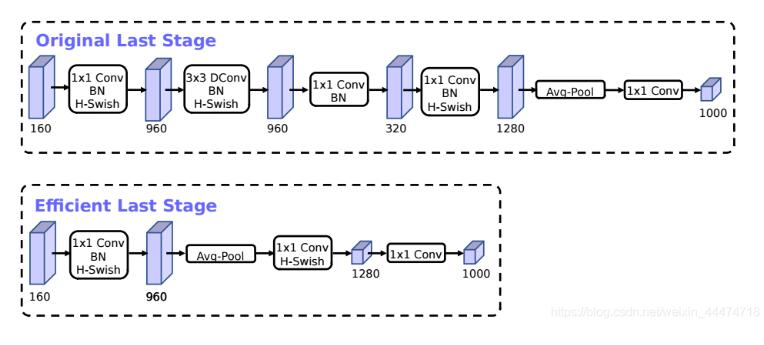
\includegraphics[width=0.5\linewidth]{webmin/网络的改进.jpg}
	\caption{V2与V3网络最后部分}
	\label{fig-bijiaojiegou}
\end{figure}

图\ref{fig-bijiaojiegou}中,上边的是v2网络的尾部结构,下边的则是v3的尾部,因为作者发现(NAS发现?)这部分的计算量很大,所以进行了简化,移除了33卷积层,将avg-pool层前移。

同时我们也可以从图中看出,每层卷积的最后用的是H-Swish激活函数,因为作者团队也发现了新出的激活函数swish\cite{2016Bridging,2018Sigmoid}可以有效的提高网络精度,其定义如下:
\begin{equation}
	\text { swish } x=x \cdot \sigma(x)
		\label{eq-swish}
\end{equation}
虽然这种非线性函数提高了精度,但在嵌入式环境中代价是非零的,因为在移动设备上计算sigmoid函数要昂贵得多,于是作者提出了解决方式:

\begin{equation}
	\mathrm{h}-\mathrm{swish}[x]=x \frac{\operatorname{ReLU} 6(x+3)}{6}
		\label{eq-hswish}
\end{equation}
相近似的激活函数也在另一篇论文中提出\cite{2019hard-swish},可以达到计算量小,而准确率相近,并且延迟还大大降低。


\begin{figure}[htbp]
	\centering
	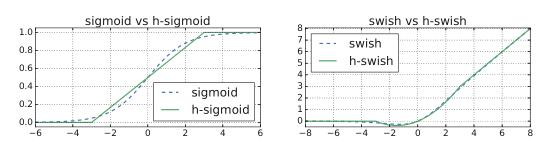
\includegraphics[width=0.7\linewidth]{webmin/sigmoid_h_sigmoid.jpg}
	\caption{两中激活函数的比较}
	\label{fig-hsish}
\end{figure}

从图中可以看出,swish和h-swish激活函数是十分相近的,而计算量和延迟却下降了。


\subsection{网络结构}
MobileNetV3被定义为两个模型:MobileNetV3大的和MobileNetV3小的。这些模型分别针对高资源和低资源用例。这些模型是通过将支持平台的NAS\cite{MnasNet}和NetAdapt\cite{NetAdapt}应用于网络搜索并结合本节中定义的网络改进而创建的。

\begin{figure}[htpb]
	\centering
		\subfigure[big]{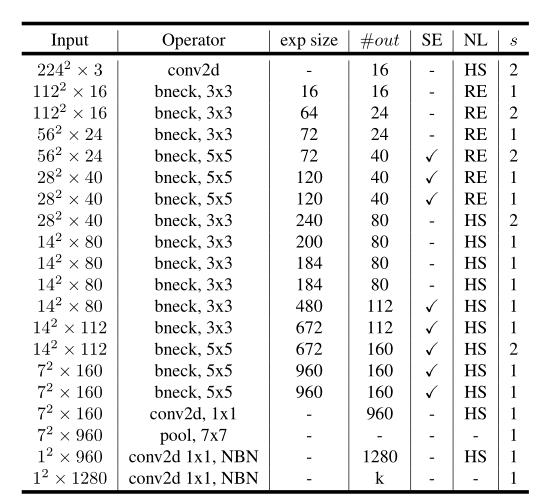
\includegraphics[width=0.4\linewidth]{webmin/bigmobv3.jpg}\label{fig-bigv3}}
	\subfigure[small]{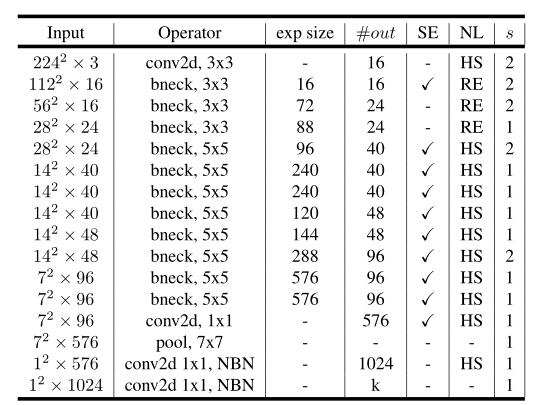
\includegraphics[width=0.4\linewidth]{webmin/smallmobv3.jpg}\label{fig-smallv3}}
	\label{fig-MobileNetV3-Large and MobileNetV3-Small}
	\caption{MobileNetV3-Large and MobileNetV3-Small}
\end{figure}

其中的bneck就是第二节中\ref{sec-v2}中应用BottleNecks。SE表示是否应用了挤压和激励\cite{MnasNet},NL表示应用的
非线性激活类型,RE表示ReLU,HS表示hard-swish激活。NBN表示不应用batch normalization。

\subsection{效果对比}
我们主要看看目标检测方面的效果对比。作者使用MobileNetV3作为SSDLite\cite{MOBV2}中主干特征提取器的替代品,并与COCO数据集上的其他主干网进行了比较\cite{COCO}。
\begin{figure}[htbp]
	\centering
	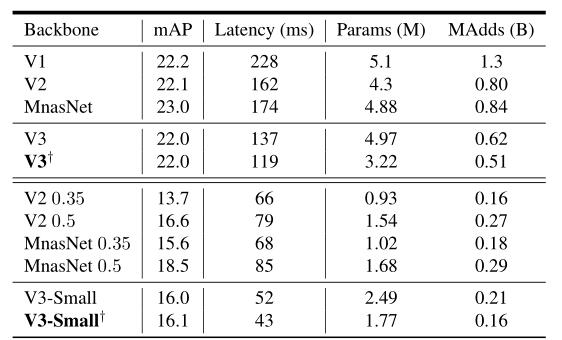
\includegraphics[width=0.7\linewidth]{webmin/v3结果比较.jpg}
	\caption{不同骨架的SSDLite在COCO测试集上的目标检测结果}
	\label{fig-v3jieguobijiao}
\end{figure}

图\ref{fig-v3jieguobijiao}中给出了COCO测试集的结果。随着信道的减少,MobileNetV3 Large比具有几乎相同mAP的MobileNetV2快27\%。MobileNetV3Small(信道缩减)map稍微低于V2和MnasNet\cite{MnasNet},但是速度却快了35\%。
\subsection{小结}
当看到MobileNetV3 应用强化学习的方法来进行网络搜索来构建网络的时候,真的感觉很惊奇,因为在学习深度学习的过程中,各种网络纷繁复杂,有时候不禁会想作者到底是怎么构建这些网络的,有时候可以找到理由,但是大部分还是无法得到其中的道理,而网络搜索技术的应用,或许真的会成为以后神经网络构建的主流吧。


\section{简单的实验}
实验方面暂时只是进行了以MobileNetV2 与 ResNet50\cite{resnet} 作为faster-RCNN\cite{23}目标检测框架的骨干网络。
\subsection{数据集}
数据集应用的并不是pascal voc数据集\cite{VOC2007}。而是华南理工大学人机智能交互实验室的提供的SCUT-Ego-Gesture Dataset\cite{YOLSE}数据集。\\
数据集地址:\url{http://www.hcii-lab.net/data/scutegogesture/}\\
SCUT-Ego-Gesture数据集是SCUT-Ego-Finger数据集的扩展。该数据集包含59111个RGB图像,这些图像包含16种不同的手势(11种单手手势和5种双手手势)。单手11种手势:单手(3374帧)、单2帧(3763帧)、单三帧(3768帧)、单四帧(3767帧)、单五帧(3755帧)、单六帧(3757帧)、单七帧(3773帧)、单八帧(3380帧)、单九帧(3769帧)、SinleBad(3761帧)、SingleGood(3769帧);双手5种手势:PairSix(3681帧)、PairSeven(3707帧)、PairEight(3653帧)、PairNine(3653帧)和PairTen(3536帧)。
数据集样本如图\ref{fig-SCUT}:
\begin{figure}[htbp]
	\centering
	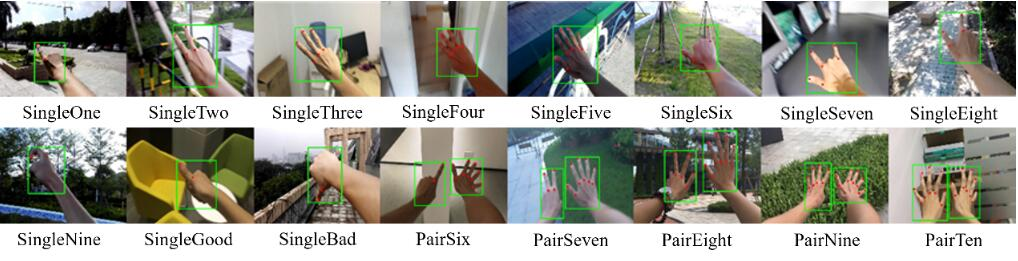
\includegraphics[width=\linewidth]{webmin/SCUT.jpg}
		
		\caption{SCUT-Ego-Gesture数据集样本}
		\label{fig-SCUT}
\end{figure}

本次实验我们仅仅提取11个单手手势数据作为训练集和验证集,训练集集为百分之70\%,验证集为剩下的百分之30\%.


\subsection{实验内容}
实验内容方面,我们主要想要验证mobilenetV2与resnet50为骨干网络时,fasterCNN的检测结果差别,Average Precision  (AP) @[ IoU=0.50:0.95 | area=   all | maxDets=100 ] 指标和Average Recall     (AR) @[ IoU=0.50:0.95 | area=   all | maxDets=100 ] 指标。

%resnetandmobilenetap.jpg
%召回率不同曲线的召回率.jpg/
%训练过程的损失曲线.jpg

\begin{table}[htbp]
	\centering
	\caption{以mobilenetv2和resnet50作为骨干网络的fasterrcnn结果比较}
	\begin{tabular}{l c c r}
		\hline\hline
	backbone 指标 & AP & RC \\
	\hline
	ResNet50 & 0.846 & 0.892 \\
	MobileNetV2& 0.833 & 0.878 \\	
	\hline
	\label{table-在手势数据集上最终得到的结果比较}
	\end{tabular}	
\end{table}

\begin{figure}[htbp]
	\centering
	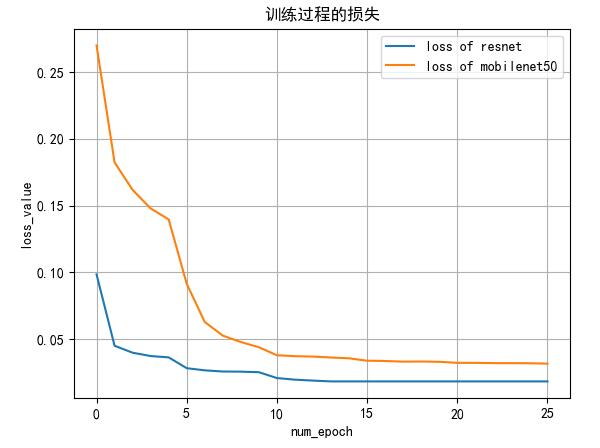
\includegraphics[width=0.5\linewidth]{webmin/训练过程的损失曲线.jpg}
	
	\caption{训练过程的loss变化曲线}
	\label{fig-loss曲线}
\end{figure}
\begin{figure}[htbp]
	\centering
	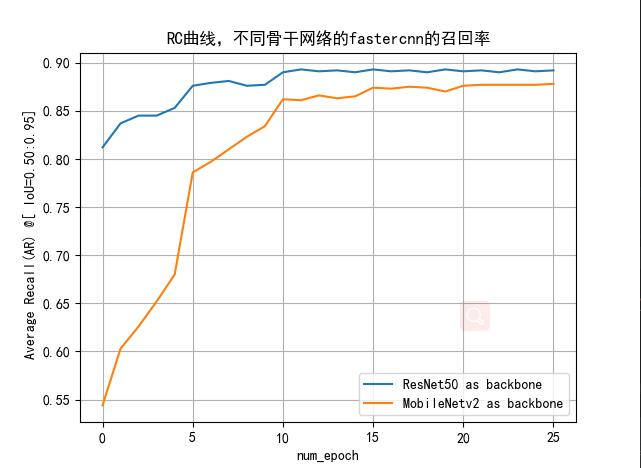
\includegraphics[width=0.5\linewidth]{webmin/召回率不同曲线的召回率.jpg}
	
	\caption{训练过程的召回率曲线}
	\label{fig-rc曲线}
\end{figure}



\begin{figure}[htbp]
	\centering
	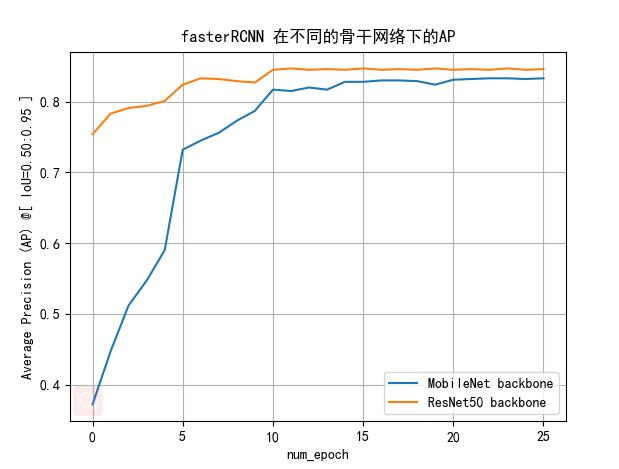
\includegraphics[width=0.5\linewidth]{webmin/resnetandmobilenetap.jpg}
	
	\caption{训练过程的AP曲线}
	\label{fig-ap曲线}
\end{figure}

我们从数据集上最终训练的结果表\ref{table-在手势数据集上最终得到的结果比较}可以看出,resNet50的效果要比用MobileNetV2的结果要好一些。

\begin{figure}[htbp]
	\centering
	\subfigure[mobileNet测试结果]{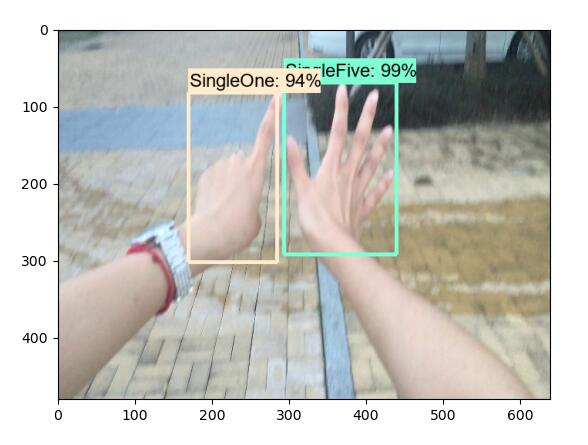
\includegraphics[width=0.4\linewidth]{webmin/mobile_pic.jpg}
		\label{fig-mobileceshi}}
	\subfigure[resnet50测试结果]{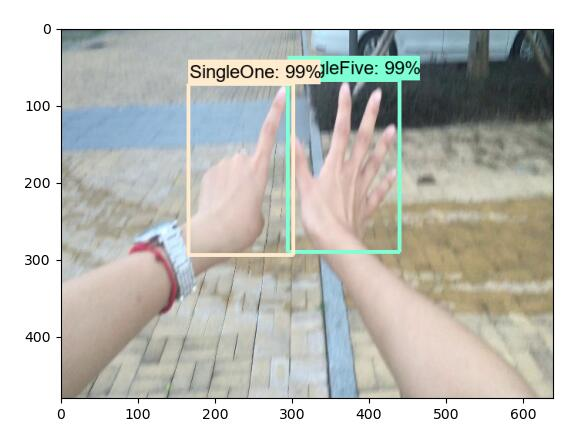
\includegraphics[width=0.4\linewidth]{webmin/resnet50ceshi.jpg}
		\label{fig-resnet50ceshi}}
	\caption{简单的效果展示}
	\label{fig_ceshixiaoguozhanshi}
\end{figure}
\subsection{还未完成的工作}
 虽然做了一些相关的工作,但是很明显,这点实验对论文中的验证还是十分不足的:\\
\begin{itemize}
	\item 无法测试mobilnetv2和resnet50在fasterrcnn上推理时间差别,因为fasterrcnn本身并不是十分快的网络,而且运算也并非几种在骨干网络,RPN,于ROIpooling层的计算量也十分大的,所以就无法测试骨干网络的推理时间的快慢了。
	\item 
	实验只是在测试了mobilenetV2,并未测试V3。
\end{itemize}
\vskip3em
\qquad 所以,接下来,还会计划实行以下计划:\\
\begin{itemize}
	\item 用ssd300,ssdlite来代替代fasterRcnn进行手势检测实验。
	\item 用mobilenetV3替换V2骨干网络,并对比效果。
\end{itemize}


%\begin{equation}\label{eq}
%  \gamma _2^{\text{C}} = \frac{{{P_{RT}}g}}{{{P_{BT}}d_{_{{B_2}2}}^{ - \alpha } + {N_0}}}
%\end{equation}
 
%插入图片
%\begin{figure}[H]   %*表示可跨栏,如果不需要可去掉
%\centering
%\subfigure[$\sum {{I_C}}  < {I_B}$]{
%  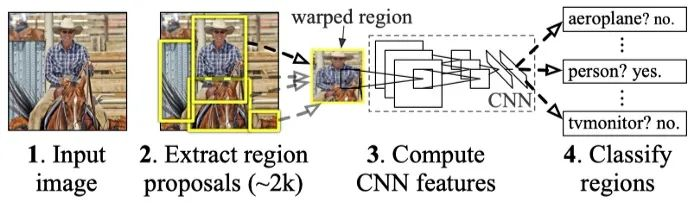
\includegraphics[width=7cm]{1.eps}}
%  %\hspace{0cm}      %两张图片之间的距离
%%\hfill               %撑满整行
%\centering
%\subfigure[$\sum {{I_C}}  > {I_B}$]{
%  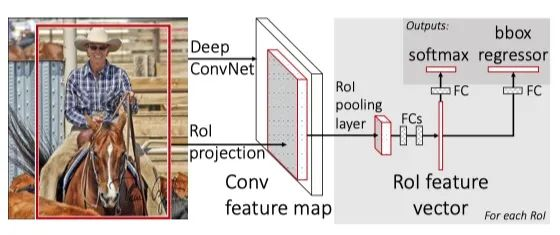
\includegraphics[width=7cm]{2.eps}}
%\caption{系统的模式选择}\label{fig}
%\end{figure}
 
%插入表格
%\begin{table}[H] \wuhao             %局部字体设置大小
%   \centering
%  \caption{系统模型符号}\label{tab}
%  \begin{tabular}{c|c}
%    \toprule                  %设置为顶线默认格式 加粗
%    % after \\: \hline or \cline{col1-col2} \cline{col3-col4} ...
%    符号 & 说明 \\
%    \hline                  %普通横线
%    ${{B_1}\mbox{、}{B_2}}$ & 基站的下标表示 \\
%    ${C_1}\mbox{、}{C_2}$ & 蜂窝用户的下标表示 \\
%    $D$ & D2D用户的下标表示 \\
%    $R$ & 中继用户的下标表示 \\
%    ${P_{it}}\left( {i = B,C,D,R} \right)$ & 终端$i$的发射功率 \\
%    ${d_{ij}}(i,j = {B_k},{C_k},1,2,R;i \ne j,k = 1,2)$ & 设备$i$到设备$j$的距离 \\
%    ${h_{ij}}(i,j = {B_k},{C_k},1,2,R;i \ne j,k = 1,2)$ &$i$-$j$ 链路的信道系数\\
%    ${n_i}\left( {{n_i}\sim N\left( {\mu ,{N_0}} \right)} \right)$ & 高斯白噪声 \\
%    ${P_{ij}} = {P_{iT}}d_{ij}^{ - \alpha }$ & 终端$j$收到的终端$i$发送的信号功率\\
%    $\alpha$ & 路径衰落系数 \\
%    \bottomrule                %设置为底线默认格式
%  \end{tabular}
%\end{table}
% 
%引用:图\ref{fig},式\eqref{eq},表\ref{tab}
 
%\section{实验与分析}



\bibliography{mob.bib}
\begin{appendices}
	\section{附录:数据集与代码地址}
	\noindent 实验数据集:\url{http://www.hcii-lab.net/data/scutegogesture/}\\
	\qquad 实验代码:\url{https://github.com/smiledinisa/-web_mining_final_work}
\end{appendices}
\end{document}
